% Template for Elsevier CRC journal article
% version 1.2 dated 09 May 2011

% This file (c) 2009-2011 Elsevier Ltd.  Modifications may be freely made,
% provided the edited file is saved under a different name

% This file contains modifications for Procedia Computer Science

% Changes since version 1.1
% - added "procedia" option compliant with ecrc.sty version 1.2a
%   (makes the layout approximately the same as the Word CRC template)
% - added example for generating copyright line in abstract

%-----------------------------------------------------------------------------------

%% This template uses the elsarticle.cls document class and the extension package ecrc.sty
%% For full documentation on usage of elsarticle.cls, consult the documentation "elsdoc.pdf"
%% Further resources available at http://www.elsevier.com/latex

%-----------------------------------------------------------------------------------

%%%%%%%%%%%%%%%%%%%%%%%%%%%%%%%%%%%%%%%%%%%%%%%%%%%%%%%%%%%%%%
%%%%%%%%%%%%%%%%%%%%%%%%%%%%%%%%%%%%%%%%%%%%%%%%%%%%%%%%%%%%%%
%%                                                          %%
%% Important note on usage                                  %%
%% -----------------------                                  %%
%% This file should normally be compiled with PDFLaTeX      %%
%% Using standard LaTeX should work but may produce clashes %%
%%                                                          %%
%%%%%%%%%%%%%%%%%%%%%%%%%%%%%%%%%%%%%%%%%%%%%%%%%%%%%%%%%%%%%%
%%%%%%%%%%%%%%%%%%%%%%%%%%%%%%%%%%%%%%%%%%%%%%%%%%%%%%%%%%%%%%

%% The '3p' and 'times' class options of elsarticle are used for Elsevier CRC
%% The 'procedia' option causes ecrc to approximate to the Word template
\documentclass[3p,times,procedia]{elsarticle}
\flushbottom

%% The `ecrc' package must be called to make the CRC functionality available
\usepackage{ecrc}
\usepackage[bookmarks=false]{hyperref}
    \hypersetup{colorlinks,
      linkcolor=blue,
      citecolor=blue,
      urlcolor=blue}
%\usepackage{amsmath}


%% The ecrc package defines commands needed for running heads and logos.
%% For running heads, you can set the journal name, the volume, the starting page and the authors

%% set the volume if you know. Otherwise `00'
\volume{00}

%% set the starting page if not 1
\firstpage{1}

%% Give the name of the journal
\journalname{Procedia Computer Science}

%% Give the author list to appear in the running head
%% Example \runauth{C.V. Radhakrishnan et al.}
\runauth{Y. Acikmese, S.E. Alptekin}

%% The choice of journal logo is determined by the \jid and \jnltitlelogo commands.
%% A user-supplied logo with the name <\jid>logo.pdf will be inserted if present.
%% e.g. if \jid{yspmi} the system will look for a file yspmilogo.pdf
%% Otherwise the content of \jnltitlelogo will be set between horizontal lines as a default logo

%% Give the abbreviation of the Journal.
\jid{procs}

%% Give a short journal name for the dummy logo (if needed)
%\jnltitlelogo{Computer Science}

%% Hereafter the template follows `elsarticle'.
%% For more details see the existing template files elsarticle-template-harv.tex and elsarticle-template-num.tex.

%% Elsevier CRC generally uses a numbered reference style
%% For this, the conventions of elsarticle-template-num.tex should be followed (included below)
%% If using BibTeX, use the style file elsarticle-num.bst

%% End of ecrc-specific commands
%%%%%%%%%%%%%%%%%%%%%%%%%%%%%%%%%%%%%%%%%%%%%%%%%%%%%%%%%%%%%%%%%%%%%%%%%%

%% The amssymb package provides various useful mathematical symbols

\usepackage{amssymb}
%% The amsthm package provides extended theorem environments
%% \usepackage{amsthm}

%% The lineno packages adds line numbers. Start line numbering with
%% \begin{linenumbers}, end it with \end{linenumbers}. Or switch it on
%% for the whole article with \linenumbers after \end{frontmatter}.
%% \usepackage{lineno}

%% natbib.sty is loaded by default. However, natbib options can be
%% provided with \biboptions{...} command. Following options are
%% valid:

%%   round  -  round parentheses are used (default)
%%   square -  square brackets are used   [option]
%%   curly  -  curly braces are used      {option}
%%   angle  -  angle brackets are used    <option>
%%   semicolon  -  multiple citations separated by semi-colon
%%   colon  - same as semicolon, an earlier confusion
%%   comma  -  separated by comma
%%   numbers-  selects numerical citations
%%   super  -  numerical citations as superscripts
%%   sort   -  sorts multiple citations according to order in ref. list
%%   sort&compress   -  like sort, but also compresses numerical citations
%%   compress - compresses without sorting
%%
%% \biboptions{authoryear}

% \biboptions{}

% if you have landscape tables
\usepackage[figuresright]{rotating}
%\usepackage{harvard}
% put your own definitions here:x
%   \newcommand{\cZ}{\cal{Z}}
%   \newtheorem{def}{Definition}[section]
%   ...

% add words to TeX's hyphenation exception list
%\hyphenation{author another created financial paper re-commend-ed Post-Script}

% declarations for front matter
\renewcommand\thepage{}  % REMOVE PAGE NUMBERS
\begin{document}
\begin{frontmatter}

%% Title, authors and addresses

%% use the tnoteref command within \title for footnotes;
%% use the tnotetext command for the associated footnote;
%% use the fnref command within \author or \address for footnotes;
%% use the fntext command for the associated footnote;
%% use the corref command within \author for corresponding author footnotes;
%% use the cortext command for the associated footnote;
%% use the ead command for the email address,
%% and the form \ead[url] for the home page:
%%
%% \title{Title\tnoteref{label1}}
%% \tnotetext[label1]{}
%% \author{Name\corref{cor1}\fnref{label2}}
%% \ead{email address}
%% \ead[url]{home page}
%% \fntext[label2]{}
%% \cortext[cor1]{}
%% \address{Address\fnref{label3}}
%% \fntext[label3]{}

\dochead{23rd International Conference on Knowledge-Based and Intelligent Information \& Engineering Systems}%
%% Use \dochead if there is an article header, e.g. \dochead{Short communication}
%% \dochead can also be used to include a conference title, if directed by the editors
%% e.g. \dochead{17th International Conference on Dynamical Processes in Excited States of Solids}

\title{Prediction of stress levels with LSTM and passive mobile sensors}

%% use optional labels to link authors explicitly to addresses:
%% \author[label1,label2]{<author name>}
%% \address[label1]{<address>}
%% \address[label2]{<address>}



\author[a]{Yasin Acikmese} 
\author[b]{S. Emre Alptekin}

\address[a, b]{Galatasaray University, Ciragan Cad. No.36, 34357 Istanbul, Turkey}


\begin{abstract}
Stress levels among people rise through the years, and passive sensing data from mobile phones or other ubiquitous devices have started to found its place in applications of mental health observation. With the ultimate goal of creating an automatic human mental health assistant that helps people to have a better mental condition, a step is taken by creating a stress recognition model. In previous works, the researchers have found correlations between sensor data and mental health conditions. They attempted to predict the stress level by different data sources. Due to there is no direct link between any sensor data with mental health, Machine Learning algorithms are employed to uncover relations with multiple sensors and mental well-being. The utilized machine learning algorithms work with non-sequence data hence the researchers need to extract features that represent historical sensor data as one value features. However, extracted features cannot completely represent time-varying sequence data. Within the scope of this study, we demonstrate that LSTM, CNN and CNN-LSTM algorithms, which accept sequence data as input can also work in passive mobile phone sensor data to predict human mental stress. The performance of the model on StudentLife dataset that includes passive mobile sensing data and stress feedbacks of college students has 62.83\% accuracy on 460 test instances by training with 800 instances with LSTM model. The diversity of the data is limited and the size is tiny for the data-hungry LSTM model. Consequently, the model could not generalize on adapted features with the small sample size. Although we did not adapt complex features, the results encourage us to improve data size and continue to research on this topic.
\end{abstract}

\begin{keyword}
recurrent neural networks, LSTM, pattern recognition, mobile sensing, stress

%% keywords here, in the form: keyword \sep keyword

%% PACS codes here, in the form: \PACS code \sep code

%% MSC codes here, in the form: \MSC code \sep code
%% or \MSC[2008] code \sep code (2000 is the default)

\end{keyword}
\cortext[cor1]{Corresponding author. Tel.: +90-212-227-4480 ; fax: +90-212-259-5557.}
\end{frontmatter}

%\correspondingauthor[*]{Corresponding author. Tel.: +0-000-000-0000 ; fax: +0-000-000-0000.}
\email{yasinacikmese@gmail.com}

%%
%% Start line numbering here if you want
%%
% \linenumbers

%% main text

%\enlargethispage{-7mm}
\section{Introduction}
\label{intro}
Stress level among people is raising with modern life \cite{Weiten2014}. Chasing success, academic and work pressures are some of the main contributors to the stress. Increased stress levels among people advance the risk of a lot of mental and physiological health problems. In the work of life stress and health review \cite{Slavich2016}, stressful life has a lot of harms to asthma, rheumatoid arthritis, anxiety disorders, depression, cardiovascular disease, chronic pain, HIV/AIDS, stroke, cancer and accelerated biological aging and premature mortality. Furthermore, deprivation of brain cells and reduced brain size \cite{Kang2012} can be related to stress. In addition to the stress caused physiological diseases that participate in people in the long-term to cause damage or even death, many psychological discomforts may lead to suicide. The latest work \cite{Liu2019} which includes 67,000 college students reveals that 75\% of students have at least one stressful time period in the past year, and 20\% of students reported that more than 5 stressful times. In the work \cite{Landow2006}, researchers reported that anxiety levels are broadening among college students. In the survey, 83 schools reported increased use of mental health services in the last three years and more than half of the schools do not know how many of the students are seeking for help. In addition to growing stress levels among people and their major effects, it is possible to take precautions such as meditation \cite{Holzel2009}\cite{Smith2013}, exercise \cite{Viveros2013}, getting enough sleep \cite{Kushlev2015}, limiting the frequency of checking email \cite{Brown2009}, yoga \cite{Cervellin2011}, listening music \cite{Rapaport2010}, massage \cite{Scholey2009} and chewing gum \cite{Fehske2011} to lessen the harms of stress. As a result of the studies that we discussed, we can note that stress can have tremendous influences on people, and the life of many people can get better with the precautions at the beginning phase of stress.
  
Every 10 years since the 70s, a new generation of computing devices have risen and the adaptation to certain computing devices has been growing. With certain advancements in every era, hardware capability of computation power grows and becomes more affordable with smaller devices. The most adapted generation of those computing devices is (smart) mobile phones \cite{ict}. They are miniature, energy efficient and highly computationally skilled devices that are in the pockets of 2 out 3 people in the world \cite{DaSilva2019}. There are a lot of sensors that are embedded in mobile phones throughout the years. With enhanced computation ability and new sensors, it becomes accessible to collect real-time data from different aspects of human life. Data-driven modeling is more focused on understanding the manner of work of the world with experiments by exploiting high-performance computation devices. Consequently, a lot of studies with mobile phones is done from human activity recognition to mental health recognition. Continuously growing personal data by ubiquitous devices that are related to activities, routines, and social interactions create a lot of new opportunities to create a better social life and to build predictive and assisting models.
  
Ultimately, our aim is to evaluate and improve human mental health conditions by utilizing behavioral data and artificially intelligent algorithms. Our focus is especially on mobile phone data and we are interested in the prediction of human mental comfort that requires response data that we predict in future cases. With respect to the point, historical data and algorithmic methods are tested. In this work, we attempt automatic recognition of daily stress with two classes ("Stressed" and "Not-Stressed") as a Machine Learning classification task which is based on passive sensor data from smartphones. The main scientific contribution of the work contains applying one of the best algorithms for sequence data (LSTM) types on daily stress recognition from passive mobile phone data. Recurrent Neural Network (RNN) and derivatives give some of the best results for sequential data in recent years. Because of the working structure of the RNN, uncovering relationships between each feature and carrying significant aspect from the beginning of the sequence to the end are the main gains. Due to our dataset have time-series features, we can generate sequences for different time periods to make it suitable to feed RNN. We explore use cases in stress recognition with Machine Learning by utilizing Recurrent Neural Network because it decreases the labor cost of feature engineering that affects the solution time in a positive manner. Here, we hypothesized that because of RNNs’ functioning structure and our input type, RNN can predict the stressful students from time-varying features set. To confirm the assumption of the appropriateness of RNN to our proposed application and stress recognition task, we used StudentLife dataset and formed an LSTM model to classify the people who are stressed or not. Other than LSTM, chosen algorithms (CNN and CNN-LSTM) are compared according to validation methods. With all features that we extracted, we reached 62.83\% accuracy on the test set with LSTM model. 
  
The rest of the paper is organized as follows; the next section introduces related works, materials and methods that are used to produce results are explained in Section 3. Classification algorithms and verification metrics are introduced in Section 4. The results and discussion are in Section 5, and the paper is concluded in Section 6.


\section{Related works}
\label{related-works}
Collecting information from the life of people for specific time periods have been obtained by daily or weekly diaries, which include thoughts and activities of a person. Still, the types of data collection in a particular time period only depend on one's memories. Even if people may remember most of the things, they cannot explain every scenario in a small time span. Besides, the data collection procedure could set a barrier because it takes an effort to complete the process. Accordingly, the data collection procedure that is entirely reliant on the efforts of humans generates small and highly biased data. 

Mobile phones have an advantage over any other data collection method. The advantage is having the ability of both passive and active data collection. Passive and active data acquisition can be accomplished via sensors and instantaneous interactions respectively. The StudentLife dataset \cite{Wang2014} was created via mobile phones with StudentLife app where sensor data and response of students to different questions are collected. Consequently, it is known when students have a bad or good mood with ecological momentary assessments (EMAs). 

In the StudentLife work \cite{Wang2014}, the relationship between passive sensor data and psychological well-being of students was checked by well-known mental health surveys. The research showed that interpersonal relationships and academic life in college are stress determinants for students. Further, because of the complexity of life that involves a lot of decisions and actions, there can be interconnected links which may not be interpreted easily with basic statistical approaches. However, the methods that use information from compounded actions and reactions may reveal hidden reasons better. There are some studies, \cite{BenZeev2015, Becker2016, Pratap2019, Saeb2016} that tried to correlate passive mobile phone sensing data with mental health conditions. These works attempted to recognize links between stress and time-varying features and predicts stress levels. 

Depressive indications were classified with 60\% sensitivity in the generalized model and 75\% sensitivity in personalized model with using 8 days time interval data \cite{Canzian2015}. There is a negative correlation between GPS data and depression \cite{Saeb2016}, and the relationship is more apparent on weekends. SVM and Random Forest reached 61\% and 59\% accuracy in the prediction of depressive traits with smartphone data \cite{Wahle2016}. Sensor and social features were used to predict the mood of the people and the result was 70\% accuracy with Markov-Chain Monte Carlo methods \cite{Ma2014}. In another work, personalized linear regression's accuracy varies between 55\% and 76\% for predicting mood. Besides, it is revealed that sleep duration and mobility are the contributors to daily life stress \cite{Ben-Zeev2015}. These results denote that there are relationships between sensor data and mental health conditions. The results vary in related to the application types; mood or stress prediction with sensor data is not highly accurate in generalized applications. These methods use algorithms that cannot recognize patterns in time have so researchers extract features to exhibit time-dependent features.


\section{Materials and methods}
\label{materials-methods}

\subsection{Dataset}
StudentLife dataset \cite{Wang2014} is used for stress recognition task. It is preferred because passive and automatic data from mobile phones are collected. The data was collected from 48 Dartmouth students for a 10-week spring term. During the data collection process, each student has an Android-based smart mobile phone in which StudentLife app (sensing and feedback software) had run 24/7 to collect automatic measurements and take feedbacks. The dataset was anonymized to secure privacy concerns of students so we worked on anonymized data.

\subsubsection{Sensor data}
The dataset carries 10 sub-directories which includes 10 different sensor data. Physical activity, audio inferences, conversation inferences, Bluetooth, light sensor, GPS, phone charge, phone lock, Wi-Fi, Wi-Fi location are the sensor data which are collected 24/7 without any interaction. GPS and Wi-Fi location data are discarded because of the collected data only contains information about a college campus. There are 4 labels for activity and audio inference. Stationary, Walking, Running and Unknown are for activity inference, and Silence, Voice, Noise and Unknown are for audio inference. For each timestamp in activity and audio data, there is a one Id information that describes the current situation of the user. Conversation classifier was used to label when the student having a conversation. If the classifier caught a conversation from audio data, it continued to accumulate conversation data until the end. Bluetooth and Wi-Fi data include signal levels of nearby devices for a specific timestamp. The light data were recorded when the phone’s light sensor could not detect light for more than 1 hour. The data of the period when the phone is locked or charged is also available.

\subsubsection{EMA data}
Responses to the EMA questions (stress reports) were acquired when the user interacts with the phone. The responses alter according to question types, some of them are multi-choice and others are user inputs. There are several questions in these self-reports, we only extracted questions and their answers that are not directly about a specific location and more generalizable to every situation in general. Hence, we only used Stress and Mood data for the stress recognition task.

\subsubsection{Other data}
To be able to use the time of the day information (day, night, and so forth), we extracted hour from the timestamp as a new feature. Consequently, the algorithm can correlate the time of the day with other features. Besides, different types of data were collected from students but we practiced educational, SMS, call log and app usage data in our model because they are time-series data. We also choose deadlines data to feed into our model. Deadlines data include homework, projects, quiz, mid-terms and finals data. They were collected daily from each student and the total values were recorded for each day. SMS data holds information about when the student sends or receives an SMS. Additionally, each student has a different file which has timestamp and call information. Likewise, call log indicates that how many calls are made or received for given timestamps. App usage data includes names and the total number of running apps.


\subsection{Preprocessing}
There are different files for each student in separate directories with respect to each type of data. The preprocessing is performed to create a dataset which contains input instances and outputs.

\subsubsection{Labels}
Labels were extracted from EMA responses which contain stress-related questions (Stress and Mood 2) (Table~1). Labels were converted in the form of binary classification ("Stressed" or "Not-Stressed"). For Stress data, selection 1-3 were converted to "Stressed" label and selection 4-5 were converted to "Not-Stressed". Similarly, we took selection 2 in Mood 2 data as "Stressed" and selection 1 as "Not-Stressed". All labels have timestamp information so we can match the labels with the right input data.

\begin{table}[h]
\caption{Label generation.}
\begin{tabular*}{\hsize}{@{\extracolsep{\fill}}lll@{}}
\toprule
Data & Stress & Mood 2\\
\colrule
Question & Right now, I am... & How are you right now?\\
Choice 1 & A little stressed & Happy\\
Choice 2 & Definitely stressed & Stressed\\
Choice 3 & Stressed out & Tired\\
Choice 4 & Feeling good\\
Choice 5 & Feeling great\\
\botrule
\end{tabular*}
\end{table}

\subsubsection{Sensor data}
Sensor data is simply stored in three ways. The first type has a value for each timestamp, the second type defines a time range for particular actions and the third type contains multiple values for a specific timestamp (Fig.~1). Therefore, the feature generation from the sensor data consists of different procedures for each data type. Activity and audio data are of the first data type; conversation, light sensor, phone charge and phone lock data are of the second data type; and Bluetooth and Wi-Fi data are of the third data type. 

When creating the feature set, timestamp information was used as the matching value in the process of joining different data. Feature set generation was started with activity data. Because of activity and audio data have only one value for specific timestamp, they were joined by the timestamp. Conversation, light sensor, phone charge and phone lock data have time range information. Therefore, new features were created for each of them by adding boolean information to the specified time range. To add new features from Bluetooth and Wi-Fi data, we did some statistical calculations to represent multiple data. Bluetooth and Wi-Fi have multiple values (signal levels) for each timestamp. Consequently, mean and standard deviation and total count were calculated for each timestamp to understand the count of nearby devices and their signal levels. After multiple data was converted to single timestamp representation by these calculations, they were added as new features.

\subsubsection{Other data}
The features used other than sensor data are deadlines, call log, running apps, SMS and hour of the day. Deadlines data includes how much total deadlines a student has for each day. Therefore, we added the deadline count to the whole day in our feature set. Call log, SMS and running app data have multiple values for a specific timestamp. We counted the total values for each timestamp to represent the total call log, SMS and running app. Then, we have added these features to our feature set according to timestamps. Lastly, the hour of the day information was attached to the feature set by extracting hour information from timestamps. The creation process of each feature from different data types can be seen in Fig.~1.

\begin{figure}[t]\vspace*{4pt}
%\centerline{\includegraphics{fx1}\hspace*{5mm}\includegraphics{fx1}}
\centerline{\includegraphics[width=110mm]{graphics/Dataset_Preparation.png}}
\caption{data types and preprocessing.}
\end{figure}

\begin{figure}[t]\vspace*{4pt}
%\centerline{\includegraphics{fx1}\hspace*{5mm}\includegraphics{fx1}}
\centerline{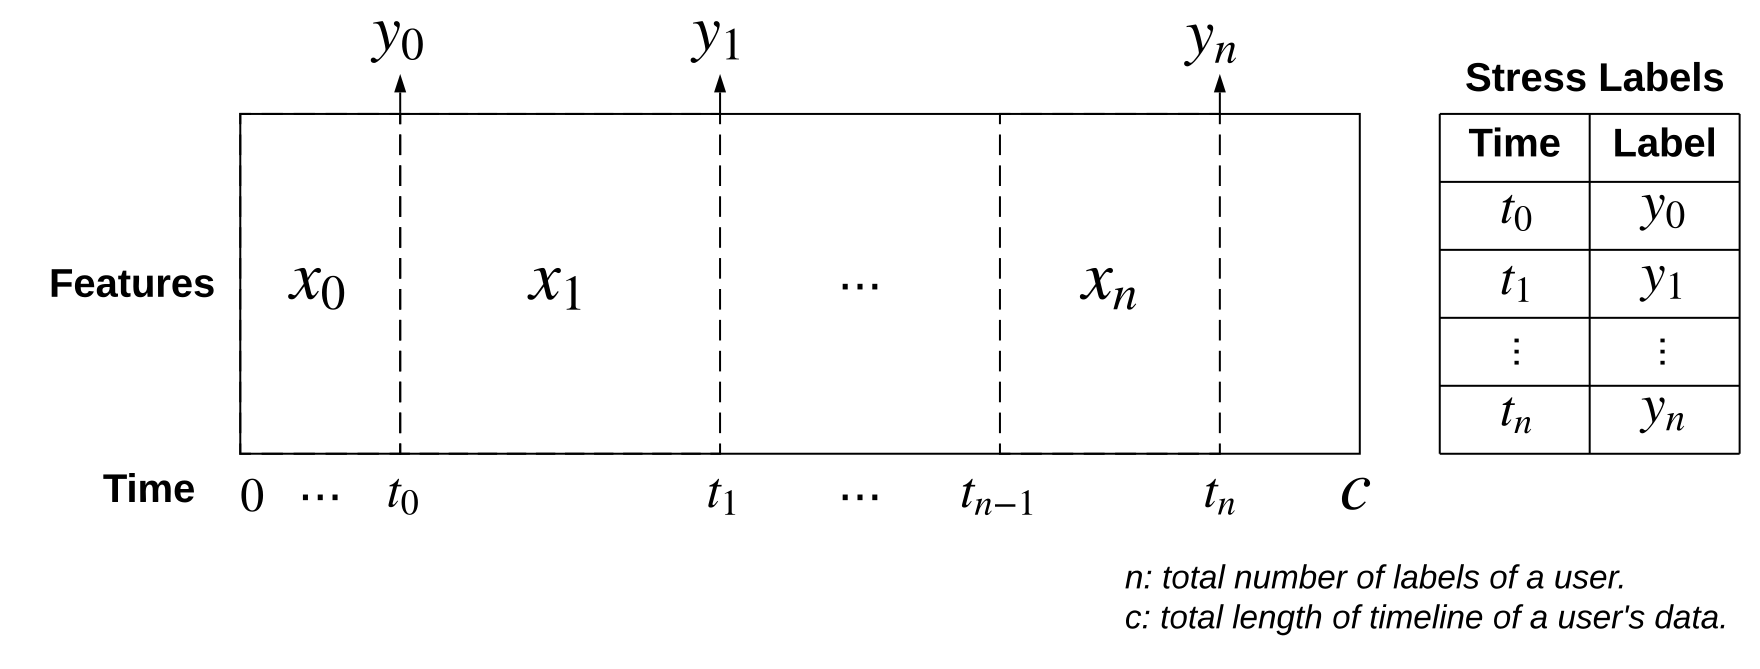
\includegraphics[width=110mm]{graphics/Creating_Instances.png}}
\caption{instance and label creation for rnn.}
\end{figure}

\subsubsection{Converting data to same length instances and adding labels}
After extracting labels from students' feedbacks, we had a label for specific timestamp for each student. Relations between timestamps, features and labels are in Fig.~2. To be able to create features as time-series, it is necessary to obtain a time interval before the specified timestamps for each label. Because of the feedback from students came after different time intervals, when we extract instances according to stress labels, some instances became too long and some short. For this reason, we have decided to look at the time span of up to 12 hours before each feedback. Therefore, while extracting instances and labels from calculated attributes, we have received data from the last 12 hours for those with a time interval of more than 12 hours, and all data for those less than 12 hours. Moreover, we did not take feedback with a time interval of less than 2 hours, we combined them with the next feedback. When creating these time-series features, we would have had a very long time series to feed the model if we had taken each moment in seconds or minutes. Hence, we re-sampled the time series in 30 minutes to eliminate very long sequences. Finally, since the length of sequences with a time span of fewer than 12 hours is not the same as the others, we have padded the forefront of the sequences with zeros using the padding method. As a result, the samples consisting of 24 units and their labels were prepared to be fed to the RNN model. 

\subsubsection{Normalization}
Data normalization is one of the most utilized data preparation processes in Neural Networks. It makes all input values in a similar range and thus makes the model can converge to optimal parameters faster. Moreover, it reduces the probability of getting stuck in the local optima and increase the probability to reach global optima. We practiced Yeo-Johnson Transformation \cite{Yeo2000} for data normalization process. It is a more complex calculation than basic normalization/transformation techniques like Min-Max scaling or log transformation but it has some advantages. If the data has non-normal distribution, we can use Box-Cox transformation or Yeo-Johnson transformation to transform data into a normal distribution. However, Yeo-Johnson allows transformation for negative data without worrying about the domain. 


\section{Classification and verification}
\label{classification}
Because of our discrete outputs, we needed to use a classification method to reach our stress recognition goal. In the classification process, the output label is known and the algorithm tries to separate data into discrete groups. Therefore, we generated 2 classes ("Stressed" and "Not-Stressed") to create a binary classification problem. Label "0" represents "Not-Stressed" and label "1" represents "Stressed" in our task.

\subsection{LSTM}
For the classification process, the model needs a mapped input instance and its output. There are different methods that can be used for classification process and most used ones are Logistic Regression, Nearest Neighbors, Naive Bayes, Support Vector Machines, Decision Trees and Artificial Neural Networks. These classification methods need each instance as one shot (fixed-size of a vector). In other words, there is no internal state getting updated in time. Therefore, if there are sequence data, we need to find a way to represent time-varying data in the shape that the model accepts. To convert time-series data to a single value, descriptive statistics such as sum, mean, standard deviation and so forth are usually calculated. Besides, there are some tools for specific domains to represent time-series data in an alternate representation such as Fourier Transformation. However, none of these methods can represent sequence data completely. There is always something missing from the data such as data dependencies.

\begin{figure}[t]\vspace*{4pt}
%\centerline{\includegraphics{fx1}\hspace*{5mm}\includegraphics{fx1}}
\centerline{\includegraphics[width=110mm]{graphics/LSTM_Cell.png}}
\caption{lstm cell.}
\end{figure}

Due to the structure of the Recurrent Neural Network (RNN), we can train a classification model without needing a preprocessing to decrease the shape of sequence features to one shot vector. Internal state in RNN models is updated in time during model training so it can identify the relationships between each sequence. We can think of RNN as multiple copies of a network in a loop and information can pass through a network to another in that loop. Hence, it can transport data from one step to another in a sequence. Natural language processing and other types of applications, which have sequence data are the areas, that utilized RNN to reach exceptional results. Nevertheless, because of the vanishing or exploding gradient problem of RNN, it can only work well on short-term dependencies \cite{Bengio1994}. Accordingly, Long Short-Term Memory (LSTM) \cite{Hochreiter1994} is emerged to solve this short-term dependency problem and make the network to remember longer dependencies. In addition to RNN structure, LSTM has a cell state, which transfers the information through LSTM cells with a minor change of the information. Consequently, the network's default behavior is to remember long-term dependencies. Furthermore, LSTM structure includes three gates, (forget gate, update gate, output gate) which decide about the information that goes to the next cell. Forget gate decides what information is eliminated, the input gate selects which values to update and output gate determines what is the output of the cell. An LSTM cell structure and LSTM data workflow can be seen in Fig.~3 and Fig.~4, respectively. Mathematical calculations of LSTM cell is at Equation~1 where $F_{i}$ is the forget gate, $I_{i}$ is the input gate and $O_{i}$ is the output gate of the cell. $x_{i}$ is the input values, $W$ with different underscores represent weight matrix of each data and underscore $i$ is for the sequence (time) in the LSTM network. $\tilde{c}_{i}$, $c_{i}$ are the update values for previous cell state and the new cell state, in respectively. $h_{i}$ represents the output of the cell.

\begin{equation}
\begin{array}{l}
{F_{i}=\sigma\left(W_{F}\left[h_{i-1}, x_{i}\right]+b_{F}\right)} \\ {I_{i}=\sigma\left(W_{I}\left[h_{i-1}, x_{i}\right]+b_{I}\right)} \\ 
{\tilde{c}_{i}=\tanh \left(W_{c}\left[h_{i-1}, x_{i}\right]+b_{c}\right)} \\ 
{c_{i}=F_{i} \circ c_{i-1}+I_{i} \circ \tilde{c}_{i}} \\ {O{i}=\sigma\left(W_{O}\left[h_{i-1}, x_{i}\right]+b_{O}\right)} \\ 
{h_{i}=O{i} \circ \tanh \left(c_{i}\right)}\end{array}
\end{equation}

To compare results with similar dataset, we choose 2 new and promising algorithms, CNN (Convolutional Neural Network) and CNN-LSTM (Convolutional Neural Network - Long Short-Term Memory) \cite{Karim2018}.

\begin{figure}[t]\vspace*{4pt}
%\centerline{\includegraphics{fx1}\hspace*{5mm}\includegraphics{fx1}}
\centerline{\includegraphics[width=110mm]{graphics/Simple_RNN.png}}
\caption{rnn workflow.}
\end{figure}

\subsection{Model architecture}
To reach the best result from the dataset, we tried different model architectures. For LSTM model, one LSTM layer with 64 nodes and 0.2 dropout rate, one fully-connected layer with 64 nodes, a dropout layer with the rate of 0.2 and one fully-connected layer with one node were used to create the structure for classification. Hyperbolic Tangent was used for activation function and the learning rate was $0.0003$. Binary cross-entropy/logarithmic loss and Adam optimizer were used for loss function and optimization in respectively.  
For CNN model, 2 convolution layers, max pooling layer, 2 convolution layers, global average pooling and a dropout layer were used. Lastly, for CNN-LSTM model, 1 convolution layer, max pooling layer, LSTM layer and full-connected layers were used. 

\subsection{Verification}
Models should uncover hidden insights from the data without memorizing the training data (overfitting). We utilized Accuracy, Precision, Recall, F1-Score and ROC-AUC to evaluate the performance of the model. We calculated these metrics to measure the performance of the model on the test set so we can observe the performance of the model on unseen data. 

\section{Results and Discussion}
Using continuous passive sensing data of college students, we are able to decide with \%62.83 confidence if the student is stressed or not by looking at their last 2-12 hours mobile sensing data. To train this model, we used 800 training instances, 200 validation instances and 460 test instances, and all of them are balanced dataset. We aimed to test LSTM, because continuous sensor data is time-varying and we thought that the LSTM algorithm is very suitable for this dataset. We can feed the time-series data as a sequence to discover relationships and dependencies between each time's feature values. In this way, it can reveal the changing behavior of users over time. Our sequence length for each instance is 24 and each member of the instance represents 30 min data which means that we look at the data of the student at most 12 hours. 

The features of the input data are activity inference, audio inference, Bluetooth, call log, conversation, deadlines, the hour of the day, phone charging, phone in the dark, phone locked, running apps and SMS. Activity inference and audio inference are categorical and they are one hot encoded to feed into the model.

The works that were done previously in similar datasets did not show very accurate results for predictive models \cite{Wang2014, DaSilva2019, Becker2016, Pratap2019}. However, they have found that there are relationships between mobile passive sensing data and stress. They were also showed that user based models outperform general models in prediction performance. Nevertheless, we created a general model, which means that the results are not for a specific student, they are valid for all students.

\begin{figure}[t]\vspace*{4pt}
%\centerline{\includegraphics{fx1}\hspace*{5mm}\includegraphics{fx1}}
\centerline{\includegraphics[width=110mm]{graphics/loss_acc.jpg}}
\caption{accuracy and loss of test data at each epoch.}
\end{figure}

Loss and accuracy graph can be seen on the Fig.~5. As we can see that our training and test loss are decreasing until specific epoch and after that point, training loss is decreasing but test loss is increasing. Consequently, we train our model until that epoch to reach our best generalizable performance. In our tests, if we increase the number of epochs, training performance reaches 99\% accuracy but test performance drops. This is a very clear indicator of overfitting and we tried different methods such as using dropout or decreasing the complexity of the model but none of them helped to solve overfitting problem. We think that this problem occurs because of the data that we have. Adding new features or expanding the size of the data with different samples may help the algorithm to discover more generalizable differences between each class. We trained 3 different models and as it is seen in the Table~3, all three models' performances are similar to each other but LSTM performs slightly better.

\begin{table}[h]
\caption{Model Metrics.}
\begin{tabular*}{\hsize}{@{\extracolsep{\fill}}llllll@{}}
\toprule
Data & Accuracy & Precision & Recall & F1-Score & Support\\
\colrule
Not-Stressed & 0.63 & 0.62 & 0.63 & 0.63 & 230 \\
Stressed & 0.63 & 0.63 & 0.63 & 0.63 & 230 \\
Average & 0.63 & 0.63 & 0.63 & 0.63 & 460 \\
\botrule
\end{tabular*}
\end{table}

\begin{table}[h]
\caption{Comparison of algorithms.}
\begin{tabular*}{\hsize}{@{\extracolsep{\fill}}llll@{}}
\toprule
Metric & LSTM & CNN & CNN-LSTM\\
\colrule
Accuracy & 62.83\% & 60.43\% & 60.00\% \\
\botrule
\end{tabular*}
\end{table}

The reason of the LSTM outperforms CNN and CNN-LSTM may be about the dataset and characteristics of algorithms. In general, CNN algorithm is more suitable for spatial data such as images and LSTM is more suitable for temporal/sequential data. CNN tries to identify patterns between neurons but RNN uncovers time-series information from input data. CNN algorithm takes fixed size inputs but LSTM can handle various input lengths because it uses its internal memory to process arbitrary sequences of inputs. Even if the two algorithms try to represent patterns, the representation mechanisms are different. CNN looks for the same patterns on all the different subfields of the input data but LSTM feeds hidden layers as input for the next step. Thus, LSTM builds a memory throughout the training although it does not look for the same patterns over different parts of the sequence. In our case, our input length varies from sample to sample, because of the time intervals between each feedback. To handle these variances, we used padding to create the same length instances to feed into the models. Because of our input lengths varies a lot, the padding process adds a lot of zeros to the front of the instances. In consequence of CNN algorithm learn from fixed size input, zeros would affect the learning performance. However, LSTM uncovers time-dependent patterns but it does not take any data from padding part because zeros do not move any information to the next sequence step. Consequently, LSTM is not affected by zeros from padding and it focuses on important parts better. For the CNN-LSTM case, CNN layer is generally used for feature extraction for LSTM layer in image and video analysis. It mostly used with pre-trained CNN layer to extract features from images. In our case, we did not use any pre-trained layer and adding one more layer increases the complexity of the model. Because of our small dataset, the more complex model may not generalize better than pure LSTM. Moreover, it could also suffer from zeros from padding during feature extraction by CNN. Consequently, even if the dataset leads to better performance with LSTM, there are not enormous differences between algorithms.

Our ultimate objective is to predict stress and orient people to have a less stressful life. There were studies that we discussed earlier were also trying to predict a person's mood or stress with different algorithms; however, we tried one of the most successful algorithms (LSTM) for time-series data in latest years to improve the performance. Even if the algorithm gave great promises for time-series application at first, our features and sample size cannot generate great results but encourage us to improve the dataset and features to reach our goal.

\section{Conclusion}
In this work, we created a model to predict the stress levels of students. Our main target is a system, that analyses human previous passive data and makes predictions about mental health conditions and gives insights about findings to users. We used StudentLife dataset, which has mobile sensing and stress feedback data from college students. We preprocessed the data to make it ready for RNN algorithm structure. Specifically, LSTM algorithm was adopted to classify "Stressed" and "Not-Stressed" students with generated features. The accuracy of the model on the balanced test set is 62.83\%. Further research will be directed to include more diverse data from people from different background. Moreover, we will collect new features to improve the model's performance. After creating a base model which has a satisfactory result, we want to adopt the online learning technique to make the model adapt to the user with new data.


\section*{Acknowledgements}
This research has been financially supported by Galatasaray University Research Fund, with the project number 19.402.007.


\begin{thebibliography}{}

\bibitem{Wang2014}
Wang, Rui, et al. (2014) ``StudentLife: assessing mental health, academic performance and behavioral trends of college students using smartphones." {\it In Proceedings of the 2014 ACM international joint conference on pervasive and ubiquitous computing}: 3--14.

\bibitem{Slavich2016}
Slavich, George M. (2016) ``Life stress and health: a review of conceptual issues and recent findings." {\it Teaching of Psychology} {\bf 43} (4): 346--355.

\bibitem{Kang2012}
Kang, Hyo Jung, et al. (2012) ``Decreased expression of synapse-related genes and loss of synapses in major depressive disorder." {\it Nature medicine} {\bf 18} (9): 1413.

\bibitem{Holzel2009}
Hölzel, Britta K., et al. (2009) ``Stress reduction correlates with structural changes in the amygdala." {\it Social cognitive and affective neuroscience} {\bf 5} (1): 11--17.

\bibitem{Smith2013}
Smith, J. C. (2013) ``Effects of emotional exposure on state anxiety after acute exercise." {\it Medicine and science in sports and exercise} {\bf 45} (2): 372--378.

\bibitem{Viveros2013}
Viveros, Jennifer, and David G. Schramm. (2018) ``Why Stress Management Strategies Work."

\bibitem{Kushlev2015}
Kushlev, Kostadin, and Elizabeth W. Dunn. (2015) ``Checking email less frequently reduces stress." {\it Computers in Human Behavior} {\bf 43}: 220--228.

\bibitem{Brown2009}
Brown, Richard P., and Patricia L. Gerbarg. (2013) ``Yoga breathing, meditation, and longevity." {\it Annals of the New York Academy of Sciences} {\bf 1172} (1): 54--62.

\bibitem{Cervellin2011}
Cervellin, Gianfranco, and Giuseppe Lippi. (2011) ``From music-beat to heart-beat: a journey in the complex interactions between music, brain and heart." {\it European journal of internal medicine} {\bf 22} (4): 371--374.

\bibitem{Rapaport2010}
Rapaport, Mark Hyman, Pamela Schettler, and Catherine Bresee. (2010) ``A preliminary study of the effects of a single session of Swedish massage on hypothalamic–pituitary–adrenal and immune function in normal individuals." {\it The Journal of Alternative and Complementary Medicine} {\bf 16} (10): 1079--1088.

\bibitem{Scholey2009}
Scholey, Andrew, Crystal Haskell, Bernadette Robertson, David Kennedy, Anthea Milne, and Mark Wetherell. (2009) ``Chewing gum alleviates negative mood and reduces cortisol during acute laboratory psychological stress." {\it Physiology & behavior} {\bf 97} (3--4): 304--312.

\bibitem{Fehske2011}
Fehske, Albrecht, Gerhard Fettweis, Jens Malmodin, and Gergely Biczok. (2011) ``The global footprint of mobile communications: The ecological and economic perspective." {\it IEEE Communications Magazine} {\bf 49} (8): 55-62.

\bibitem{BenZeev2015}
Ben-Zeev, Dror, Emily A. Scherer, Rui Wang, Haiyi Xie, and Andrew T. Campbell. (2015) ``Next-generation psychiatric assessment: Using smartphone sensors to monitor behavior and mental health." {\it Psychiatric rehabilitation journal} {\bf 38} (3): 218.

\bibitem{Bengio1994}
Bengio, Yoshua, Patrice Simard, and Paolo Frasconi. (1994) ``Learning long-term dependencies with gradient descent is difficult." {\it IEEE transactions on neural networks} {\bf 5} (2): 157--166.

\bibitem{Hochreiter1994}
Hochreiter, Sepp, and Jürgen Schmidhuber. (1994) ``Long short-term memory." {\it Neural computation} {\bf 9} (8): 1735--1780.

\bibitem{Karim2018}
Karim, Fazle, Somshubra Majumdar, Houshang Darabi, and Shun Chen. (2018) ``LSTM fully convolutional networks for time series classification." {\it IEEE Access} {\bf 6}: 1662-1669.

\bibitem{Yeo2000}
Yeo, In‐Kwon, and Richard A. Johnson. (2000) ``A new family of power transformations to improve normality or symmetry." {\it Biometrika} {\bf 87} (4): 954-959.

\bibitem{DaSilva2019}
DaSilva, Alex W., Jeremy F. Huckins, Rui Wang, Weichen Wang, Dylan D. Wagner, and Andrew T. Campbell. (2019) ``Correlates of Stress in the College Environment Uncovered by the Application of Penalized Generalized Estimating Equations to Mobile Sensing Data." {\it JMIR mHealth and uHealth} {\bf 7} (3): e12084.

\bibitem{Becker2016}
Becker, Dennis, Vincent Bremer, Burkhardt Funk, Joost Asselbergs, Heleen Riper, and Jeroen Ruwaard. (2016) ``How to predict mood? Delving into features of smartphone-based data."

\bibitem{Pratap2019}
Pratap, Abhishek, David C. Atkins, Brenna N. Renn, Michael J. Tanana, Sean D. Mooney, Joaquin A. Anguera, and Patricia A. Areán. (2019) ``The accuracy of passive phone sensors in predicting daily mood." {\it Depression and anxiety} {\bf 36} (1): 72-81.

\bibitem{Canzian2015}
Canzian, Luca, and Mirco Musolesi. (2015) ``Trajectories of depression: unobtrusive monitoring of depressive states by means of smartphone mobility traces analysis." {\it n Proceedings of the 2015 ACM international joint conference on pervasive and ubiquitous computing}: 1293-1304.

\bibitem{Saeb2016}
Saeb, Sohrab, Emily G. Lattie, Stephen M. Schueller, Konrad P. Kording, and David C. Mohr. (2016) ``The relationship between mobile phone location sensor data and depressive symptom severity." {\it PeerJ} {\bf 4}: e2537.

\bibitem{Wahle2016}
Wahle, Fabian, Tobias Kowatsch, Elgar Fleisch, Michael Rufer, and Steffi Weidt. (2016) ``Mobile sensing and support for people with depression: a pilot trial in the wild." {\it JMIR mHealth and uHealth} {\bf 4} (3): e111.

\bibitem{Ma2014}
Ma, Yuanchao, Bin Xu, Yin Bai, Guodong Sun, and Run Zhu. (2014) ``Infer Daily Mood using Mobile Phone Sensing." {\it Adhoc & Sensor Wireless Networks} {\bf 20}.

\bibitem{Ben-Zeev2015}
Ben-Zeev, Dror, Rui Wang, Saeed Abdullah, Rachel Brian, Emily A. Scherer, Lisa A. Mistler, Marta Hauser, John M. Kane, Andrew Campbell, and Tanzeem Choudhury. (2015) ``Mobile behavioral sensing for outpatients and inpatients with schizophrenia." {\it Psychiatric services} {\bf 67} (5): 558-561.

\bibitem{Liu2019}
Liu, Cindy H., Courtney Stevens, Sylvia HM Wong, Miwa Yasui, and Justin A. Chen. (2019) ``The prevalence and predictors of mental health diagnoses and suicide among US college students: Implications for addressing disparities in service use." {\it Depression and anxiety} {\bf 36} (1): 8-17.

\bibitem{Landow2006}
Landow, Mery V. (2006) ``Stress and mental health of college students" {\it Nova Publishers}.

\bibitem{Weiten2014}
Weiten, Wayne, Dana S. Dunn, and Elizabeth Yost Hammer. (2014) ``Psychology applied to modern life: Adjustment in the 21st century." {\it Cengage Learning}.

\bibitem{ict}
Sanou, Brahima. (2016) `ICT facts and figures 2016." {\it International telecommunications union, Geneva}.

\end{thebibliography}

\end{document}
